\documentclass[conference]{IEEEtran}
\IEEEoverridecommandlockouts

\usepackage[utf8]{inputenc}
\usepackage[T1]{fontenc}
\usepackage[brazilian]{babel}
\usepackage{amsmath,amssymb,amsfonts}
\usepackage{algorithmic}
\usepackage{graphicx}
\usepackage{textcomp}
\usepackage{xcolor}
\usepackage{listings}
\usepackage{url}
\usepackage{booktabs}

\lstset{
  basicstyle=\ttfamily\scriptsize,
  breaklines=true,
  columns=fullflexible,
  frame=single,
  framesep=2pt,
  xleftmargin=3pt,
  xrightmargin=3pt,
  captionpos=b
}

\def\BibTeX{{\rm B\kern-.05em{\sc i\kern-.025em b}\kern-.08em
    T\kern-.1667em\lower.7ex\hbox{E}\kern-.125emX}}

\begin{document}
\shorthandoff{"}
\renewcommand{\abstractname}{Resumo}
\renewcommand{\IEEEkeywordsname}{Palavras-chave}
\renewcommand{\refname}{Referências}

\title{FinFlow: uma Linguagem de Domínio Específico para Modelagem de Operações Financeiras\\
\large *Trabalho prático final da disciplina de Teoria da Computação e Compiladores}

\author{
\IEEEauthorblockN{Guilherme Augusto Scaglia, João Pedro Denardo, Pedro Henrique Oliveira de Souza}
\IEEEauthorblockA{
RA: 111598, RA: 113036, RA: 113364\\
\textit{Engenharia da Computação} \\
Fundação Hermínio Ometto (FHO) \\
Araras, SP, Brasil \\
\{scaglia, denardo749, pedro1204\}@alunos.fho.edu.br}
}

\maketitle

\begin{abstract}
A gestão de operações financeiras é hoje predominantemente implementada em planilhas ou em linguagens de propósito geral, ambas com limitações para expressar regras de negócio de forma auditável e acessível a especialistas de domínio. Este trabalho apresenta a FinFlow, uma linguagem de domínio específico (DSL) para modelagem financeira, com tipos nativos ao domínio (\texttt{moeda}, \texttt{percentual}) e estruturas de controle \texttt{se/senao}, \texttt{para} e \texttt{escolha}. O compilador foi implementado integralmente em Python com a ferramenta PLY: análise léxica formalizada como Autômato Finito Determinístico, análise sintática por gramática LALR(1) com 29 produções e 68 estados sem conflitos, análise semântica com tabela de símbolos e regras de tipo, e interpretador por percurso da árvore sintática. Experimentos sobre a própria gramática mostram que a escolha da tabela de precedência determina entre 0 e 9 conflitos \textit{shift/reduce} e que a ausência de conflitos não garante a semântica correta. Nove testes automatizados, seis programas de exemplo e um \textit{benchmark} com programas de até 2000 linhas validam o comportamento e mostram custo linear por fase. A integração com a API pública do Banco Central permanece como trabalho futuro.
\end{abstract}

\begin{IEEEkeywords}
Linguagem de domínio específico. Compiladores. Análise sintática. Sistema de tipos. Modelagem financeira.
\end{IEEEkeywords}

\begingroup\footnotesize\noindent\textbf{FinFlow: a Domain-Specific Language for Financial Operations Modeling}\par\smallskip
\noindent\textit{\textbf{Abstract}---}Financial operations are mostly implemented in spreadsheets or general-purpose languages, both of which struggle to express business rules in an auditable way that domain experts can read. This paper presents FinFlow, a domain-specific language (DSL) for financial modeling with domain-native types (\texttt{moeda}, i.e., money, and \texttt{percentual}, i.e., percentage) and control structures (\texttt{if/else}, \texttt{for}, \texttt{switch}). The compiler was implemented in Python with the PLY tool: lexical analysis formalized as a Deterministic Finite Automaton, an LALR(1) grammar with 29 productions and 68 states and no conflicts, semantic analysis with a symbol table and typing rules, and a tree-walking interpreter. Experiments on the grammar show that the precedence table determines between 0 and 9 shift/reduce conflicts, and that the absence of conflicts does not guarantee correct semantics. Nine automated tests, six example programs and a benchmark with programs of up to 2000 lines validate the behavior and show linear cost per phase. Integration with the Central Bank of Brazil public API remains future work.\par\smallskip
\noindent\textit{\textbf{Keywords}}---Domain-specific language. Compilers. Parsing. Type system. Financial modeling.\par
\endgroup

\section{Introdução}

A gestão de operações financeiras --- cálculo de juros, categorização de despesas, simulação de fluxo de caixa --- é hoje predominantemente implementada por meio de planilhas eletrônicas ou de linguagens de propósito geral (GPL --- \textit{General Purpose Language}), como Python, Java ou C\#. Ambas as abordagens carregam limitações estruturais que motivam este trabalho.

Planilhas dificultam a auditoria de regras de negócio: uma fórmula complexa, distribuída por dezenas de células, não possui histórico de versões nativo, é difícil de testar isoladamente e não deixa explícito \textit{por que} determinado cálculo foi feito daquela forma. Já as GPLs resolvem o problema de auditabilidade (o código pode ser versionado e testado), mas criam um gargalo diferente: exigem conhecimento técnico de programação para qualquer alteração de regra, distanciando o especialista de domínio --- o analista financeiro, que entende \textit{o que} precisa ser calculado --- de quem efetivamente implementa \textit{como} isso é calculado.

Há ainda um problema mais sutil, que motiva diretamente uma decisão de projeto: a confusão entre grandezas de naturezas distintas. Em uma GPL, um valor monetário e uma taxa percentual são ambos apenas números de ponto flutuante; nada impede, sintaticamente, somar reais a uma taxa, produzindo um resultado numericamente válido, porém financeiramente incorreto. A Seção~\ref{sec:tipagem} discute por que esse problema é conhecido na literatura e como a FinFlow o trata.

O cenário de aplicação é ancorado em dados reais. O Banco Central do Brasil disponibiliza, pelo Sistema Gerenciador de Séries Temporais (SGS), indicadores como Selic e IPCA sem necessidade de autenticação; desde março de 2025, porém, consultas por período são limitadas a dez anos e a recuperação dos últimos valores a vinte registros [1]. Aplicações sobre esses dados precisam, portanto, lidar com séries temporais estruturadas. Nesta versão do trabalho o compilador está concluído e a ingestão desses dados é prevista como camada desacoplada (Seção~\ref{sec:conclusao}).

A contribuição é tripla: (i) demonstrar que uma DSL com tipos nativos ao domínio captura, em tempo de análise, uma classe de erros financeiros que GPLs não detectam; (ii) documentar formalmente, com base na teoria de autômatos e de análise LALR, cada decisão de projeto do compilador; e (iii) reportar medições feitas sobre a implementação: experimento de precedência sobre a gramática real, catálogo de erros, suíte de testes e custo por fase em função do tamanho do programa. O restante do artigo organiza-se assim: a Seção~\ref{sec:fund} apresenta a fundamentação teórica; a Seção~\ref{sec:met} descreve a linguagem e o compilador; a Seção~\ref{sec:res} traz os resultados; e a Seção~\ref{sec:conclusao} conclui.

\section{Fundamentação Teórica e Trabalhos Relacionados}
\label{sec:fund}

A arquitetura da linguagem fundamenta-se em seis trabalhos, cobrindo desde a metodologia de decisão sobre DSLs e a teoria clássica de compiladores até o precedente mais direto de linguagem formal para o domínio financeiro.

\subsection{Como um Compilador Entende um Programa}
\label{sec:visao}

Esta subseção explica, sem pressupor conhecimento prévio de compiladores, o que o trabalho faz. Um \textbf{compilador} (ou, de forma mais geral, um processador de linguagem) é um programa que lê um texto escrito em uma linguagem de programação e o transforma em algo executável ou o executa diretamente. Uma analogia útil é a leitura de uma frase em português, que passa por quatro verificações: (1) \textit{reconhecer as palavras} (``saldo'' e ``taxa'' existem; ``\$\$'' não é uma palavra); (2) \textit{conferir a estrutura da frase} (sujeito, verbo e complemento na ordem certa); (3) \textit{conferir o sentido} (``somar laranjas com quilômetros'' é gramaticalmente possível, mas não faz sentido); e (4) \textit{agir conforme o que a frase diz}. Cada verificação corresponde a uma fase do compilador da FinFlow: análise léxica, sintática, semântica e execução (Fig.~\ref{fig:arq}).

Para ilustrar, considere uma única linha de um programa FinFlow, em que \texttt{saldo} vale R\$ 1000,00 e \texttt{taxa} vale 5\%:
\begin{minipage}{\columnwidth}\begin{lstlisting}
saldo = saldo + taxa * saldo;
\end{lstlisting}\end{minipage}\par\smallskip
O compilador a processa em quatro etapas:
\begin{enumerate}
\item \textbf{Léxica.} O texto é quebrado em unidades chamadas \textit{tokens}: o nome \texttt{saldo}, o sinal \texttt{=}, o nome \texttt{saldo}, o sinal \texttt{+}, o nome \texttt{taxa}, o sinal \texttt{*}, o nome \texttt{saldo} e o ponto e vírgula.
\item \textbf{Sintática.} Os tokens são organizados em uma árvore que respeita as regras de precedência da matemática: a multiplicação é agrupada antes da soma, ou seja, \texttt{taxa * saldo} é calculado primeiro (Fig.~\ref{fig:ast}).
\item \textbf{Semântica.} O compilador consulta uma tabela com o tipo de cada variável: \texttt{saldo} é \texttt{moeda} e \texttt{taxa} é \texttt{percentual}. Como \texttt{percentual} $\times$ \texttt{moeda} resulta em \texttt{moeda}, e \texttt{moeda} $+$ \texttt{moeda} também, a linha é aceita. Se a linha fosse \texttt{saldo + taxa}, seria recusada, pois somar reais com uma taxa não faz sentido.
\item \textbf{Execução.} Com os valores atuais, calcula-se $0{,}05 \times 1000 = 50$ e depois $1000 + 50 = 1050$, e o saldo passa a valer R\$ 1050,00.
\end{enumerate}
O restante do artigo detalha cada uma dessas etapas e as decisões técnicas por trás delas. Os termos técnicos usados estão reunidos no glossário (Tabela~\ref{tab:glossario}).

\subsection{Padrões de Decisão para DSLs}

Mernik, Heering e Sloane [2] sistematizam quando e como desenvolver uma DSL, propondo padrões de decisão, análise, projeto e implementação. Os padrões de decisão orientam a escolha entre uma linguagem dedicada e o reaproveitamento de uma GPL, considerando a maturidade do domínio, a frequência de mudança das regras e o público-alvo. \textbf{Aplicação ao nosso trabalho:} o domínio financeiro básico é maduro e bem compreendido; as regras mudam com frequência relativamente alta (taxas, políticas, categorias); e o público-alvo pretendido, analistas financeiros, tipicamente não programa. Os três critérios apontam na mesma direção, o perfil de domínio que os autores identificam como propício a uma DSL. Os padrões de implementação, por sua vez, discutem o custo de construir a linguagem do zero (\textit{compiler/interpreter}) em contraste com a embutir em uma hospedeira, tema da subseção seguinte.

\subsection{DSL Interna versus Externa}

Van Deursen, Klint e Visser [3] distinguem DSLs \textit{internas} (embutidas como biblioteca em uma linguagem hospedeira) das \textit{externas} (com sintaxe e compilador próprios). \textbf{Nossa decisão:} optou-se pela abordagem externa. O motivo é técnico: uma DSL interna em Python herdaria a tipagem dinâmica da hospedeira, na qual a distinção entre \texttt{moeda} e \texttt{percentual} só poderia ser verificada em tempo de execução, e herdaria também toda a sintaxe de Python, expondo ao analista construções irrelevantes ao domínio. Uma DSL externa, com gramática e análise semântica próprias, permite que a verificação ocorra \textit{antes} da execução. O custo dessa escolha é ter de construir todo o front-end, o que é, simultaneamente, o objetivo pedagógico da disciplina.

\subsection{Teoria Clássica de Análise Léxica e Sintática}

O tratamento formal do front-end segue Aho et al. [4], que definem a análise léxica como a construção de um Autômato Finito Determinístico (AFD) reconhecedor de expressões regulares, e a análise sintática ascendente como a construção de um autômato de pilha determinístico a partir da coleção de itens LR da gramática. Essa formulação é usada diretamente nas Seções~\ref{sec:lexico} e~\ref{sec:sintatico} para descrever, de modo formal e não apenas informal, o funcionamento do lexer e do parser da FinFlow gerados pelo PLY. Do mesmo livro vem a organização em fases (léxica, sintática, semântica, execução) adotada na Fig.~\ref{fig:arq}.

\subsection{Panorama de Ferramentas para DSLs}

Kosar, Bohra e Mernik [5] conduziram um mapeamento sistemático da literatura sobre DSLs. Entre os achados relevantes aqui, os autores observam que geradores de analisadores como ANTLR, JavaCUP e YACC produzem apenas o parser, de modo que o analisador semântico precisa ser escrito manualmente, e que, entre os estudos que informam o padrão de implementação, a abordagem por compilador aparece em 28,1\% e a por interpretador em 7,9\%. Isso é coerente com a escolha da FinFlow: um gerador de parser da família Lex/Yacc (o PLY) para o front-end, com análise semântica e interpretador escritos à mão (Seção~\ref{sec:gramatica}).

\subsection{Composicionalidade em Linguagens Financeiras}

Peyton Jones, Eber e Seward [6] introduzem uma biblioteca de combinadores que descreve contratos financeiros complexos como composições de contratos simples, com semântica denotacional composicional. \textbf{Diferencial técnico:} a FinFlow cobre um subconjunto bem mais restrito do problema (expressões aritméticas, comparações e controle de fluxo sobre valores monetários e percentuais) e não modela contratos. O princípio de composicionalidade, porém, é herdado: a produção de \texttt{expressao} é recursiva, permitindo cálculos arbitrariamente complexos a partir de operações primitivas, e o tipo de uma expressão é função dos tipos de suas subexpressões (Seção~\ref{sec:semantica}).

\subsection{Tipagem de Domínio e Prevenção de Erros}
\label{sec:tipagem}

Kennedy [7] demonstrou que unidades de medida físicas podem ser codificadas como disciplina de tipos em sistemas de inferência Hindley--Milner sem comprometer a decidibilidade da inferência. O caso mais citado para justificar esse tipo de verificação é a perda da sonda \textit{Mars Climate Orbiter}, em 1999, causada pela confusão entre libras-força e newtons entre módulos de software distintos [7]. \textbf{Posicionamento crítico:} \texttt{moeda} e \texttt{percentual} são, para o domínio financeiro, o que newtons e libras-força são para a engenharia aeroespacial: grandezas que parecem intercambiáveis por serem ambas numéricas, mas que não devem ser combinadas sem conversão explícita. A FinFlow implementa uma forma simplificada dessa disciplina --- sem inferência polimórfica, apenas com tipos fixos e uma tabela de compatibilidade --- suficiente para o escopo atual e formalizada na Seção~\ref{sec:semantica}.

\subsection{Glossário de Termos}
\label{sec:glossario}

\begin{table}[!htbp]
\caption{Glossário}
\label{tab:glossario}
\centering
\footnotesize
\begin{tabular}{@{}p{0.27\columnwidth}p{0.65\columnwidth}@{}}
\toprule
\textbf{Termo} & \textbf{Significado} \\
\midrule
DSL & linguagem de domínio específico: criada para um assunto restrito (aqui, finanças) \\
GPL & linguagem de propósito geral (Python, Java, C\#) \\
Compilador & programa que traduz ou processa um texto em linguagem de programação \\
Interpretador & programa que executa o código diretamente, sem traduzi-lo antes para outra forma \\
Token & menor unidade com significado: nome, número, operador \\
Lexer & fase que quebra o texto em tokens \\
Parser & fase que confere a estrutura e monta a árvore \\
AFD & autômato finito determinístico: máquina de estados que reconhece palavras de um tipo \\
Gramática & conjunto de regras que define quais sentenças são válidas \\
LALR(1) & técnica de análise ascendente que decide cada passo olhando um símbolo adiante \\
AST & árvore sintática abstrata: representação do programa em árvore \\
Tabela de símbolos & registro do nome e do tipo de cada variável \\
Conflito \textit{shift/reduce} & situação em que a gramática permite duas ações e o parser precisa escolher \\
Precedência & ordem de prioridade dos operadores ($*$ antes de $+$) \\
Selic / IPCA & taxa básica de juros / índice oficial de inflação do Brasil \\
SGS & sistema de séries temporais do Banco Central \\
PLY & biblioteca Python que gera lexer e parser \\
\bottomrule
\end{tabular}
\end{table}

\section{Desenvolvimento e Metodologia}
\label{sec:met}

O desenvolvimento seguiu cinco etapas, correspondentes às fases do compilador (Fig.~\ref{fig:arq}): (A) definição da gramática formal, (B) escolha de ferramentas, (C) análise léxica, (D) análise sintática e (E) análise semântica e execução. O código possui 528 linhas Python em quatro módulos (\texttt{lexer}, \texttt{parser}, \texttt{semantica}, \texttt{interpretador}), mais uma interface de linha de comando e a suíte de testes. Cada fase consome a saída da anterior e levanta erro próprio, de modo que um defeito no programa-fonte é sempre reportado pela primeira fase capaz de detectá-lo, com o número da linha.

\begin{figure*}[!t]
\centering
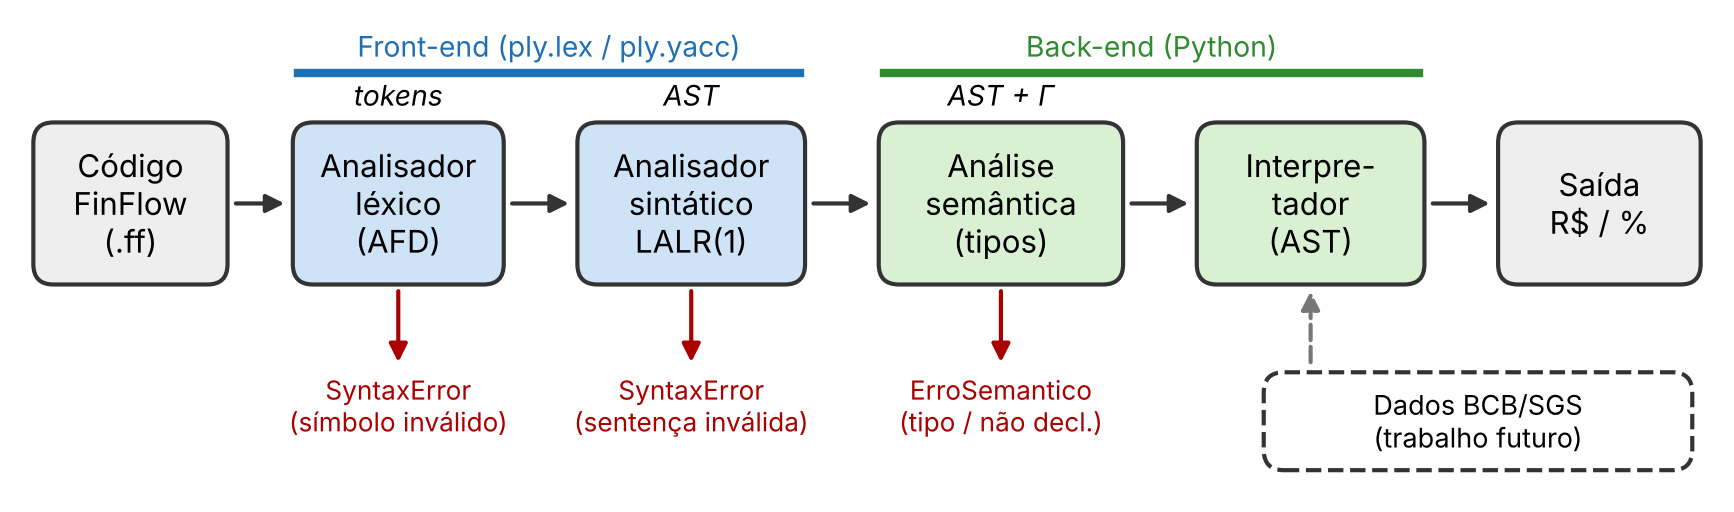
\includegraphics[width=0.88\textwidth]{fig/fig_arquitetura.png}
\caption{Arquitetura do compilador FinFlow. Erros são levantados na fase em que são detectáveis, sempre antes da execução.}
\label{fig:arq}
\end{figure*}

\subsection{A Linguagem FinFlow}
\label{sec:linguagem}

Um programa FinFlow é uma sequência de comandos terminados em ponto e vírgula. Há quatro tipos de dado: \texttt{moeda} (valor monetário, literal com ponto decimal, como \texttt{1000.00}), \texttt{percentual} (literal com sufixo, como \texttt{5\%}, armazenado como \texttt{0.05}), \texttt{inteiro} e \texttt{texto}. Os comandos são declaração, atribuição, \texttt{imprimir}, condicional (\texttt{se}/\texttt{entao}/\texttt{senao}), repetição (\texttt{para}/\texttt{ate}/\texttt{faca}) e seleção múltipla (\texttt{escolha}/\texttt{caso}/\texttt{padrao}). As três últimas estruturas atendem ao requisito da disciplina de suportar \textit{if}, \textit{for} e \textit{switch}. As palavras-chave são em português para reduzir a distância entre o analista e o código. O trecho a seguir calcula o saldo após um período de juros e decide a mensagem a exibir:
\begin{minipage}{\columnwidth}\begin{lstlisting}
moeda saldo = 1000.00;
percentual taxa = 5%;
moeda saldo_final = saldo + saldo * taxa;
se saldo_final > 1000 entao {
    imprimir("cresceu");
} senao {
    imprimir("nao cresceu");
}
imprimir(saldo_final);
\end{lstlisting}\end{minipage}\par\smallskip
Decisões de projeto relevantes: blocos delimitados obrigatoriamente por chaves, o que elimina por construção o problema do \textit{else} pendente; o laço \texttt{para} tem limite superior inclusivo e variável de controle implicitamente \texttt{inteiro}; e \texttt{escolha} executa apenas o primeiro \texttt{caso} cujo valor coincide com o alvo, sem \textit{fall-through}, evitando uma classe comum de erros de C.

\subsection{Gramática Formal e Ferramentas}
\label{sec:gramatica}

A gramática é $G = (V_N, V_T, P, S)$, em que $V_N$ é o conjunto de não-terminais, $V_T$ o de terminais (tokens do analisador léxico), $P$ o de produções e $S = \texttt{programa}$ o símbolo inicial. O \texttt{yacc} contabiliza $|P| = 29$ produções, incluindo a regra aumentada $S' \rightarrow \texttt{programa}$ (a gramática propriamente dita tem 28). Em EBNF:

\begin{minipage}{\columnwidth}\begin{lstlisting}[basicstyle=\ttfamily\fontsize{6.2}{7.2}\selectfont]
programa   ::= comando { comando }
comando    ::= declaracao | atribuicao | imprimir
             | condicional | repeticao | selecao
declaracao ::= tipo ID "=" expressao ";"
tipo       ::= "moeda" | "percentual"
             | "inteiro" | "texto"
atribuicao ::= ID "=" expressao ";"
imprimir   ::= "imprimir" "(" expressao ")" ";"
condicional::= "se" expressao "entao" bloco
               [ "senao" bloco ]
repeticao  ::= "para" ID "=" expressao "ate"
               expressao "faca" bloco
selecao    ::= "escolha" expressao "{"
               caso {caso} "}"
caso       ::= "caso" expressao ":"
               comando {comando}
             | "padrao" ":" comando {comando}
bloco      ::= "{" comando { comando } "}"
expressao  ::= expressao op_soma expressao
             | expressao op_mult expressao
             | expressao op_rel expressao
             | "(" expressao ")" | ID | CTE_INT
             | CTE_FLOAT | CTE_PERCENTUAL
             | CTE_STRING
op_soma ::= "+" | "-"
op_mult ::= "*" | "/"
op_rel  ::= "==" | "!=" | ">" | "<"
          | ">=" | "<="
\end{lstlisting}\end{minipage}\par\smallskip

As 29 produções, numeradas conforme a saída do \texttt{yacc} (usadas na Seção~\ref{sec:sintatico}), são:
\begin{minipage}{\columnwidth}\begin{lstlisting}
 1 programa -> lista_comandos
 2 lista_comandos -> lista_comandos comando
 3 lista_comandos -> comando
 4 comando -> tipo ID ATR expressao FIM_CMD
 5 comando -> ID ATR expressao FIM_CMD
 6 comando -> SE expressao ENTAO bloco
 7 comando -> SE expressao ENTAO bloco SENAO bloco
 8 comando -> IMPRIMIR ABRE_P expressao FECHA_P FIM_CMD
 9 comando -> PARA ID ATR expressao ATE expressao
              FACA bloco
10 comando -> ESCOLHA expressao ABRE_F lista_casos
              FECHA_F
11 lista_casos -> lista_casos caso | 12 caso
13 caso -> CASO expressao DOISPONTOS lista_comandos
14 caso -> PADRAO DOISPONTOS lista_comandos
15 bloco -> ABRE_F lista_comandos FECHA_F
16-19 tipo -> TIPO_MOEDA|TIPO_PERCENTUAL|
              TIPO_INTEIRO|TIPO_TEXTO
20 expressao -> expressao OP_SOMA expressao
21 expressao -> expressao OP_MULT expressao
22 expressao -> expressao OP_REL expressao
23 expressao -> ABRE_P expressao FECHA_P
24-28 expressao -> ID|CTE_INT|CTE_FLOAT|
              CTE_PERCENTUAL|CTE_STRING
\end{lstlisting}\end{minipage}\par\smallskip

Duas propriedades merecem registro. Primeiro, as listas são recursivas à esquerda (\texttt{lista\_comandos $\rightarrow$ lista\_comandos comando}), forma preferida em análise ascendente porque consome pilha constante, ao contrário da recursão à direita. Segundo, a produção de \texttt{expressao} é ambígua em uma gramática livre de contexto: a cadeia \texttt{saldo + taxa * saldo} admite duas árvores de derivação. Optou-se por manter a gramática compacta, com uma produção por categoria de operador, e resolver a ambiguidade por tabela de precedência, em vez de estratificar a gramática em níveis (\texttt{termo}, \texttt{fator}); a consequência desse caminho é medida na Seção~\ref{sec:precexp}.

A ferramenta escolhida foi o PLY (\textit{Python Lex-Yacc}) [8], em vez de ANTLR (Java) ou Flex/Bison (C/C++), por três fatores: (i) pertencer à família Lex/Yacc, cujos geradores de parser são citados no mapeamento de Kosar, Bohra e Mernik [5]; (ii) ser a ferramenta adotada na disciplina, na qual o analisador léxico é escrito pelos próprios alunos; e (iii) manter as regras próximas da notação EBNF, pois cada produção é uma docstring de função Python. O desenvolvimento ocorreu inicialmente em \textit{notebooks} e foi migrado para um projeto Python autônomo, executável por linha de comando.

\subsection{Análise Léxica: Formalização como Autômato Finito}
\label{sec:lexico}

Cada categoria de token é reconhecida por um AFD $M = (Q, \Sigma, \delta, q_0, F)$, em que $Q$ é o conjunto finito de estados, $\Sigma$ o alfabeto de entrada, $\delta : Q \times \Sigma \rightarrow Q$ a função de transição, $q_0$ o estado inicial e $F \subseteq Q$ o conjunto de estados de aceitação [4]. A Fig.~\ref{fig:afd} mostra o AFD do token \texttt{CTE\_PERCENTUAL}, de expressão regular \texttt{\textbackslash d+(\textbackslash.\textbackslash d+)?\%}: $q_1$ lê a parte inteira, $q_2$ registra o ponto decimal, $q_3$ lê a parte fracionária e $q_4$, alcançado pelo símbolo \texttt{\%}, é o estado de aceitação. Qualquer transição sem aresta em $\delta$ --- por exemplo, dois pontos decimais consecutivos --- rejeita a cadeia.

\begin{figure}[!htbp]
\centering
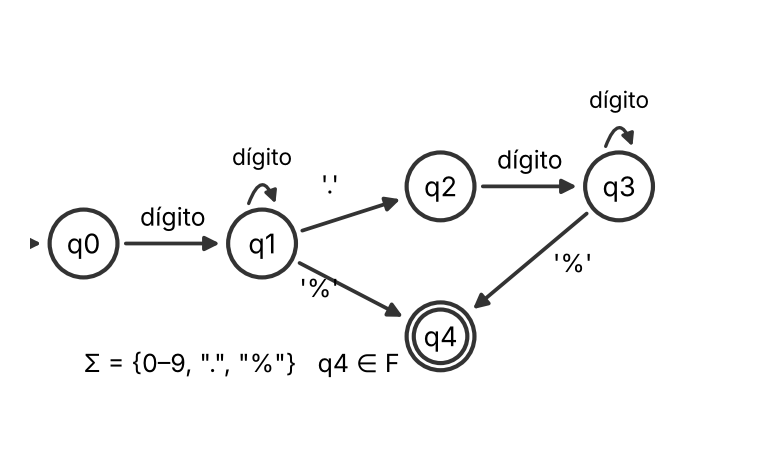
\includegraphics[width=0.95\columnwidth]{fig/fig_afd.png}
\caption{AFD do token \texttt{CTE\_PERCENTUAL}. O estado $q_4$ é de aceitação.}
\label{fig:afd}
\end{figure}

O lexer da FinFlow reconhece 16 categorias de token e 17 palavras reservadas (Tabela~\ref{tab:tokens}). Duas decisões de engenharia merecem justificativa.

\textbf{Ordem das regras.} O PLY tenta as funções de token na ordem de definição. Por isso \texttt{CTE\_PERCENTUAL} precede \texttt{CTE\_FLOAT}, que precede \texttt{CTE\_INT}: se a ordem fosse inversa, \texttt{5\%} seria lido como o inteiro 5 seguido de um símbolo inválido, e \texttt{1.5} como \texttt{1}, símbolo inválido, \texttt{5}. Em termos de AFD, a ordem implementa a escolha do lexema mais específico quando um prefixo é aceito por mais de um autômato.

\textbf{Palavras reservadas por dicionário.} Palavras como \texttt{se}, \texttt{para} e \texttt{escolha} não recebem AFD próprio; são distinguidas por consulta a um dicionário Python dentro da função do token \texttt{ID}. Se cada palavra-chave fosse uma expressão regular independente, todas competiriam com \texttt{ID} pela mesma entrada, e um identificador como \texttt{moedas} poderia ser reconhecido como a palavra \texttt{moeda} seguida de \texttt{s} por sobreposição de prefixo. Com o dicionário, o lexer lê sempre o identificador maximal e só depois decide sua categoria. Um efeito colateral é que palavras reservadas, como \texttt{e}, não podem ser usadas como nome de variável.

Os literais são convertidos ainda no lexer: \texttt{5\%} torna-se \texttt{0.05}, \texttt{1000.00} torna-se \texttt{float} e cadeias perdem as aspas. Isso antecipa para a fase léxica um trabalho que de outra forma recairia sobre o interpretador. Como traço de execução, o código \texttt{saldo = saldo + taxa * saldo;} é decomposto em \texttt{ID}, \texttt{ATR}, \texttt{ID}, \texttt{OP\_SOMA}, \texttt{ID}, \texttt{OP\_MULT}, \texttt{ID}, \texttt{FIM\_CMD}, e o literal \texttt{5\%} produz \texttt{CTE\_PERCENTUAL} com valor 0.05. Símbolos fora do alfabeto levantam \texttt{SyntaxError} com a linha (por exemplo, \texttt{Lexema invalido: '\$' na linha 1}).

\begin{table}[!htbp]
\caption{Tokens da FinFlow}
\label{tab:tokens}
\centering
\footnotesize
\begin{tabular}{@{}p{0.34\columnwidth}p{0.58\columnwidth}@{}}
\toprule
\textbf{Categoria} & \textbf{Lexemas / padrão} \\
\midrule
Literais & \texttt{CTE\_INT}, \texttt{CTE\_FLOAT}, \texttt{CTE\_PERCENTUAL}, \texttt{CTE\_STRING} \\
Identificador & \texttt{ID}: \texttt{[a-zA-Z\_][a-zA-Z0-9\_]*} \\
Operadores & \texttt{OP\_SOMA} (\texttt{+ -}), \texttt{OP\_MULT} (\texttt{* /}), \texttt{OP\_REL} (\texttt{== != > < >= <=}), \texttt{ATR} (\texttt{=}) \\
Delimitadores & \texttt{( ) \{ \} ; , :} \\
Tipos & \texttt{moeda}, \texttt{percentual}, \texttt{inteiro}, \texttt{texto} \\
Controle & \texttt{se}, \texttt{entao}, \texttt{senao}, \texttt{para}, \texttt{ate}, \texttt{faca}, \texttt{escolha}, \texttt{caso}, \texttt{padrao} \\
Outras & \texttt{imprimir}; \texttt{e}, \texttt{ou}, \texttt{nao} (reservadas, sem uso na gramática atual) \\
\bottomrule
\end{tabular}
\end{table}

\subsection{Análise Sintática: LALR(1) e Precedência de Operadores}
\label{sec:sintatico}

O \texttt{ply.yacc} constrói um parser LALR(1) (\textit{Look-Ahead LR}, com um símbolo de \textit{lookahead}). A partir da coleção canônica de itens da gramática, estados com o mesmo núcleo (itens LR(0) sem o \textit{lookahead}) são fundidos, preservando os conjuntos de \textit{lookahead} combinados. O resultado é um autômato de pilha determinístico muito menor que o LR(1) canônico equivalente, ao custo de poder introduzir conflitos \textit{reduce/reduce} em gramáticas patológicas --- o que não ocorre na FinFlow. O parser opera com uma pilha de estados e executa, a cada passo, uma de duas ações consultando a tabela com o estado do topo e o próximo token: \textit{shift} (empilha o token e avança) ou \textit{reduce} (desempilha o corpo de uma produção e empilha seu lado esquerdo). Para a gramática da Seção~\ref{sec:gramatica}, a tabela possui 68 estados.

A ambiguidade aritmética manifesta-se como conflito \textit{shift/reduce}: ao ter \texttt{expressao OP\_MULT expressao} no topo da pilha e \texttt{OP\_SOMA} como próximo token, o parser precisa decidir entre reduzir ou empilhar. O \texttt{yacc} resolve o conflito consultando uma tabela de precedência e associatividade:
\begin{minipage}{\columnwidth}\begin{lstlisting}
precedence = (('left','OP_REL'),
              ('left','OP_SOMA'),
              ('left','OP_MULT'))
\end{lstlisting}\end{minipage}\par\smallskip
Linhas posteriores têm precedência maior. A regra de decisão é: se a precedência da produção a reduzir for maior que a do próximo token, reduz; se for menor, empilha; se forem iguais, a associatividade desempata (\texttt{left} favorece a redução). Para que \texttt{+}/\texttt{-} e \texttt{*}/\texttt{/} sejam níveis distintos, o token único \texttt{OP\_ART} da primeira versão foi dividido em \texttt{OP\_SOMA} e \texttt{OP\_MULT}. A Seção~\ref{sec:precexp} quantifica o efeito dessa decisão. Os nós da árvore sintática abstrata (AST) são tuplas que carregam o número da linha, usado pelas fases seguintes nas mensagens de erro. A Fig.~\ref{fig:ast} mostra a AST de \texttt{saldo = saldo + taxa * saldo;} produzida pelo parser real.

\begin{figure}[!htbp]
\centering
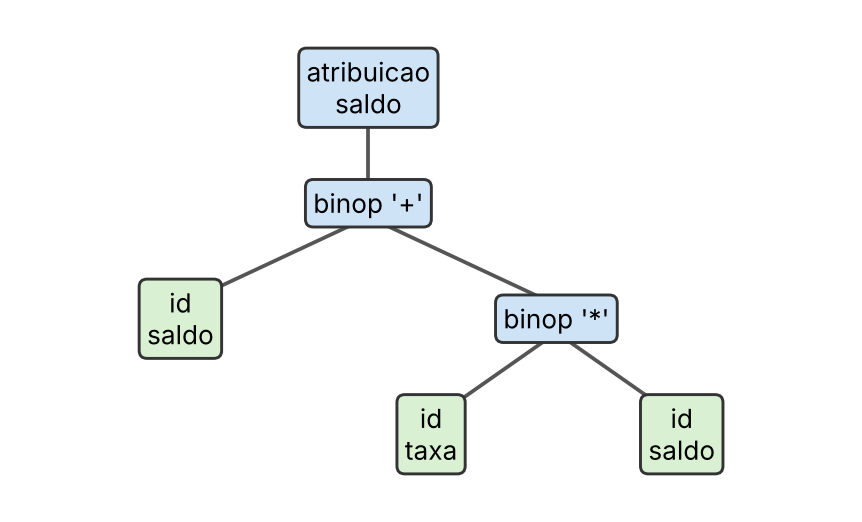
\includegraphics[width=0.85\columnwidth]{fig/fig_ast.png}
\caption{AST produzida pelo parser para \texttt{saldo = saldo + taxa * saldo;} (números de linha omitidos).}
\label{fig:ast}
\end{figure}

\textbf{Traço de análise.} A Tabela~\ref{tab:traco} reproduz o traço real do parser (modo de depuração do PLY) para \texttt{r = a + b * c;}, abreviando \texttt{expressao} por $E$. O passo 8 é onde a precedência atua: com $E$ \texttt{OP\_SOMA} $E$ na pilha (estado 41) e \texttt{OP\_MULT} como \textit{lookahead}, o parser faz \textit{shift}, adiando a soma; no passo 12, com \texttt{;} como \textit{lookahead}, a mesma configuração leva a \textit{reduce}. É essa escolha dependente do \textit{lookahead} que posiciona a multiplicação mais abaixo na árvore. O fim da análise reduz sucessivamente as produções 5, 3 e 1 e aceita a entrada.

\begin{table}[!htbp]
\caption{Traço LALR(1) de \texttt{r = a + b * c;} (parcial)}
\label{tab:traco}
\centering
\footnotesize
\begin{tabular}{@{}rp{0.40\columnwidth}ll@{}}
\toprule
\textbf{\#} & \textbf{Pilha} & \textbf{Lookahead} & \textbf{Ação} \\
\midrule
3 & \texttt{ID ATR} & \texttt{ID(a)} & shift 19 \\
4 & \texttt{ID ATR ID} & \texttt{+} & reduce 24 \\
5 & \texttt{ID ATR $E$} & \texttt{+} & shift 30 \\
7 & \texttt{ID ATR $E$ + ID} & \texttt{*} & reduce 24 \\
\textbf{8} & \texttt{ID ATR $E$ + $E$} & \texttt{*} & \textbf{shift 31} \\
10 & \texttt{ID ATR $E$ + $E$ * ID} & \texttt{;} & reduce 24 \\
11 & \texttt{ID ATR $E$ + $E$ * $E$} & \texttt{;} & reduce 21 \\
\textbf{12} & \texttt{ID ATR $E$ + $E$} & \texttt{;} & \textbf{reduce 20} \\
13 & \texttt{ID ATR $E$} & \texttt{;} & shift 38 \\
14 & \texttt{ID ATR $E$ ;} & \texttt{\$} & reduce 5 \\
\bottomrule
\end{tabular}
\end{table}

Erros sintáticos (por exemplo, \texttt{moeda x = ;}) são reportados com o token inesperado e a linha: \texttt{Erro sintatico: token inesperado 'FIM\_CMD' (';') na linha 1}. Não há recuperação de erros; o primeiro erro interrompe a compilação, o que é adequado a programas curtos.

\subsection{Análise Semântica}
\label{sec:semantica}

A análise semântica é um percurso \textit{bottom-up} da AST com uma tabela de símbolos $\Gamma$, implementada como dicionário \texttt{\{nome: (tipo, valor)\}}, formalizada por regras de inferência $\Gamma \vdash e : \tau$ (sob o contexto $\Gamma$, a expressão $e$ tem tipo $\tau$):
\begin{align}
&\frac{\Gamma \vdash e_1 : \texttt{moeda} \quad \Gamma \vdash e_2 : \texttt{moeda}}{\Gamma \vdash e_1 + e_2 : \texttt{moeda}} \\
&\frac{\Gamma \vdash e_1 : \texttt{moeda} \quad \Gamma \vdash e_2 : \texttt{percentual}}{\Gamma \vdash e_1 * e_2 : \texttt{moeda}} \\
&\frac{\Gamma \vdash e_1 : \texttt{moeda} \quad \Gamma \vdash e_2 : \texttt{percentual}}{\Gamma \vdash e_1 + e_2 : \textbf{erro}}
\end{align}
A terceira regra não produz tipo válido, e portanto a soma direta é rejeitada. A Tabela~\ref{tab:tipos} resume as combinações aceitas, extraídas das tabelas de compatibilidade do código. Literais inteiros são aceitos em comparações, atribuições e operações com \texttt{moeda} e \texttt{percentual} (por exemplo, \texttt{saldo > 1000}), por ergonomia: exigir \texttt{1000.00} em toda comparação tornaria a linguagem verbosa sem ganho de segurança, ao passo que a proibição de \texttt{moeda + percentual} é preservada. Um literal com ponto decimal é sempre tipado como \texttt{moeda}.

\begin{table}[!htbp]
\caption{Compatibilidade de Tipos nos Operadores}
\label{tab:tipos}
\centering
\footnotesize
\begin{tabular}{@{}lll@{}}
\toprule
\textbf{Operandos} & \textbf{$+$ $-$} & \textbf{$*$ $/$} \\
\midrule
moeda, moeda & moeda & moeda \\
moeda, percentual & \textbf{erro} & moeda \\
percentual, percentual & percentual & percentual \\
moeda, inteiro & moeda & moeda \\
percentual, inteiro & percentual & percentual \\
inteiro, inteiro & inteiro & inteiro \\
texto, qualquer & erro & erro \\
\bottomrule
\end{tabular}
\end{table}

Além dos operadores, a análise verifica: variável usada antes de declarada; redeclaração; atribuição de tipo incompatível; condição de \texttt{se} que não seja comparação; limites de \texttt{para} não inteiros; e tipo do \texttt{caso} diferente do tipo do alvo em \texttt{escolha}. Todas as mensagens carregam a linha do comando. As funções de análise e execução aceitam opcionalmente uma tabela e um ambiente iniciais, ponto de extensão que permitirá injetar variáveis vindas de fontes externas sem que o programador as redeclare.

\subsection{Interpretador}
\label{sec:interp}

Após a validação, um interpretador percorre a AST (\textit{tree-walking interpreter}) e executa os comandos diretamente, sem gerar código intermediário. A função de avaliação é recursiva sobre as expressões, o que reflete a composicionalidade da gramática; os comandos \texttt{para} e \texttt{escolha} usam, respectivamente, um laço sobre o intervalo inclusivo e uma busca linear pelo primeiro \texttt{caso} igual ao alvo, recorrendo ao bloco \texttt{padrao} quando nenhum coincide. Como a análise semântica já garantiu a consistência de tipos, o interpretador não repete verificações: ele confia na invariante de que um programa que chegou à execução está bem tipado. Valores são formatados conforme o tipo estático da expressão impressa (\texttt{R\$ 1050.00}, \texttt{5.00\%}). O núcleo da avaliação de expressões é, em essência:
\begin{minipage}{\columnwidth}\begin{lstlisting}
def avaliar(expr, amb):
    if expr[0] == 'id':     return amb[expr[1]]
    if expr[0].startswith('cte'): return expr[1]
    if expr[0] == 'binop':
        e = avaliar(expr[2], amb)
        d = avaliar(expr[3], amb)
        return OPS[expr[1]](e, d)   # + - * / == ...
\end{lstlisting}\end{minipage}\par\smallskip
Optou-se por interpretar a AST, em vez de gerar código, porque o escopo dos programas-alvo é pequeno e a simplicidade facilita a manipulação da linguagem e do compilador, objetivo explícito da disciplina.

\subsection{Projeto da Integração com a API SGS (não implementada)}

A integração com os dados do Banco Central foi projetada como camada desacoplada, fora do compilador, pois buscar e formatar dados externos é infraestrutura de apoio e não parte da análise léxica, sintática ou semântica. A camada consultaria o endpoint público do SGS (séries 4390, Selic acumulada no mês, e 433, variação mensal do IPCA, ambas em percentual ao mês), converteria cada valor mensal de texto para número e calcularia a variação acumulada do período pelo produto composto $\prod_i (1 + v_i/100) - 1$, e não pela soma simples, que subestima o acumulado. A série 432, por sua vez, é a meta Selic diária em percentual ao ano e não deve ser composta mensalmente. Os resultados entrariam no programa como variáveis \texttt{percentual} pré-declaradas, via os parâmetros opcionais de tabela e ambiente iniciais já existentes (e já cobertos por um teste). Com isso, o rendimento real de uma aplicação seria expresso na própria FinFlow pela relação de Fisher, $(1+i)/(1+\pi) - 1$, em que $i$ é a taxa nominal e $\pi$ a inflação. Como o SGS limita consultas a dez anos e os últimos valores a vinte registros, a camada deve tratar esses limites e levantar erro claro quando a API falhar. Nada disso foi implementado ou avaliado; é registrado apenas como decisão de projeto.

\section{Resultados e Discussão}
\label{sec:res}

\subsection{Validação por Exemplos}

Três programas de exemplo exercitam o pipeline completo (Fig.~\ref{fig:exec}), e outros três ilustram casos de uso adiante. Em \texttt{juros.ff}, o saldo de R\$ 1000,00 com taxa de 5\% resulta em R\$ 1050,00, a condição \texttt{saldo\_final > 1000} é verdadeira e o programa imprime \texttt{cresceu}. Em \texttt{para\_escolha.ff}, o laço \texttt{para} soma de 1 a 5 (resultado 15) e o \texttt{escolha} seleciona o ramo \texttt{caso 2}, imprimindo \texttt{risco moderado}. Em \texttt{erro\_tipo.ff}, a soma de \texttt{moeda} com \texttt{percentual} é rejeitada na análise semântica, com mensagem que aponta a linha e sugere a operação correta (multiplicação), antes de qualquer execução.

\begin{figure}[!htbp]
\centering
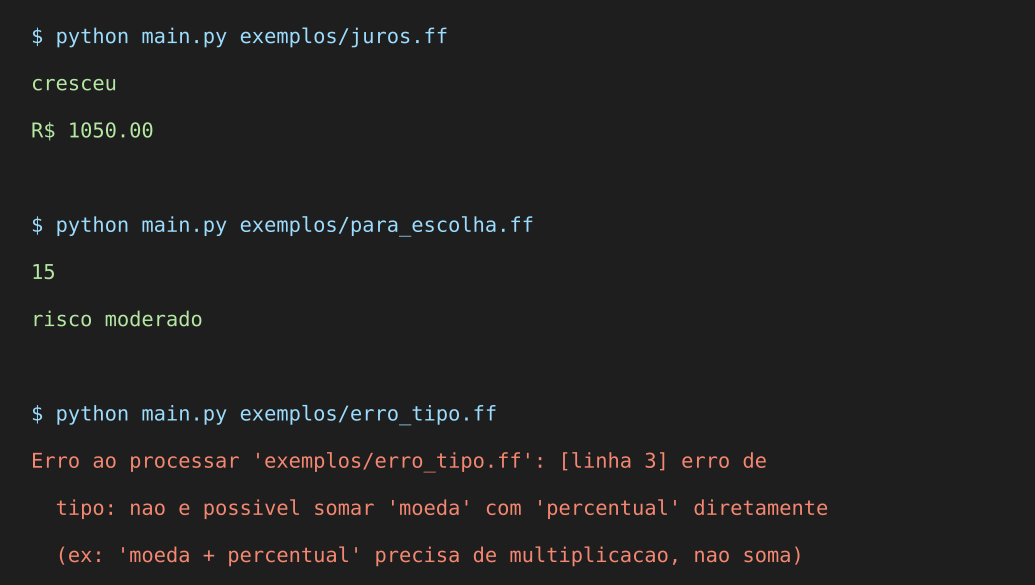
\includegraphics[width=\columnwidth]{fig/fig_execucao.png}
\caption{Saída real dos exemplos: execução correta (verde) e erro de tipo detectado estaticamente (vermelho).}
\label{fig:exec}
\end{figure}

\subsection{Exemplo com Laço: Juros Compostos}

Um quarto programa, escrito para este artigo, aplica a taxa de 1\% ao mês durante 12 meses sobre R\$ 1000,00 usando \texttt{para}, e testa uma meta com \texttt{se}:
\begin{minipage}{\columnwidth}\begin{lstlisting}
moeda saldo = 1000.00;
percentual taxa = 1%;
para mes = 1 ate 12 faca {
    saldo = saldo + saldo * taxa;
}
imprimir(saldo);
se saldo > 1100 entao { imprimir("meta atingida"); }
\end{lstlisting}\end{minipage}\par\smallskip
A execução imprime \texttt{R\$ 1126.83} e \texttt{meta atingida}, valor idêntico ao da fórmula fechada $1000 \cdot 1{,}01^{12} \approx 1126{,}83$. O exemplo mostra a vantagem expressiva da DSL: a regra de negócio (\textit{aplicar a taxa a cada mês}) é legível sem conhecimento de programação, e a análise semântica garante, antes de rodar, que \texttt{saldo * taxa} combina \texttt{moeda} com \texttt{percentual} de forma válida.

\subsection{Exemplos de Casos de Uso Financeiros}

Dois programas adicionais exploram padrões comuns do domínio. O primeiro categoriza uma despesa: um \texttt{escolha} associa a categoria a um limite de gasto, e um \texttt{se} compara a despesa ao limite.
\begin{minipage}{\columnwidth}\begin{lstlisting}
inteiro categoria = 2;
moeda gasto = 350.00;
moeda limite = 0.00;
escolha categoria {
    caso 1: limite = 200.00;
    caso 2: limite = 300.00;
    padrao: limite = 100.00;
}
se gasto > limite entao {
    imprimir("acima do limite");
} senao { imprimir("dentro do limite"); }
imprimir(limite);
\end{lstlisting}\end{minipage}\par\smallskip
A saída é \texttt{acima do limite} e \texttt{R\$ 300.00}: o \texttt{caso 2} foi selecionado e a despesa de R\$ 350,00 excede o limite. O segundo simula uma meta de poupança com aporte mensal de R\$ 250,00 e rendimento de 2\% ao mês durante seis meses:
\begin{minipage}{\columnwidth}\begin{lstlisting}
moeda poupado = 0.00;
moeda aporte = 250.00;
percentual rendimento = 2%;
inteiro meses = 0;
para m = 1 ate 6 faca {
    poupado = poupado + aporte;
    poupado = poupado + poupado * rendimento;
    meses = meses + 1;
}
imprimir(meses);  imprimir(poupado);
se poupado > 1500 entao {
    imprimir("meta de 1500 atingida");
} senao { imprimir("meta nao atingida"); }
\end{lstlisting}\end{minipage}\par\smallskip
A execução imprime \texttt{6}, \texttt{R\$ 1608.57} e \texttt{meta de 1500 atingida}. O valor foi conferido contra um cálculo independente em Python puro (1608,5708...), coincidindo até a segunda casa decimal. Os dois programas usam, em conjunto, todas as estruturas de controle da linguagem e todos os tipos de dado numéricos.

\subsection{Caracterização dos Programas de Exemplo}

A Tabela~\ref{tab:exemplos} caracteriza os seis programas distribuídos com o projeto. As contagens de tokens e de nós da AST foram obtidas executando o próprio lexer e parser; o tempo é a mediana de 50 execuções do pipeline de análise sintática, análise semântica e execução. Todos os programas completam em menos de 0,3 ms. No caso de \texttt{erro\_tipo.ff}, o tempo é menor porque o pipeline termina na análise semântica, sem chegar à execução, o que evidencia na prática que o erro é detectado cedo e a um custo mínimo. Programas maiores têm mais nós em proporção ao número de tokens, pois cada comando de controle gera nós adicionais para condição e blocos.

\begin{table}[!htbp]
\caption{Programas de Exemplo (medidos)}
\label{tab:exemplos}
\centering
\footnotesize
\setlength{\tabcolsep}{3pt}\begin{tabular}{@{}lrrrr@{}}
\toprule
\textbf{Programa} & \textbf{Linhas} & \textbf{Tokens} & \textbf{Nós AST} & \textbf{Tempo (ms)} \\
\midrule
\texttt{erro\_tipo.ff} & 3 & 17 & 9 & 0,04 \\
\texttt{juros.ff} & 9 & 44 & 21 & 0,14 \\
\texttt{juros\_comp.ff} & 7 & 44 & 22 & 0,16 \\
\texttt{para\_escolha.ff} & 11 & 57 & 27 & 0,19 \\
\texttt{categoria\_desp.ff} & 14 & 64 & 30 & 0,16 \\
\texttt{meta\_poupanca.ff} & 16 & 79 & 38 & 0,27 \\
\bottomrule
\end{tabular}
\end{table}

\subsection{Suíte de Testes}

A suíte \texttt{pytest} do compilador (\texttt{testes/test\_finflow.py}) possui 9 testes, todos aprovados (Tabela~\ref{tab:testes}). Os testes das camadas de integração e de interface (\texttt{test\_bcb.py} e \texttt{test\_playground.py}, 22 testes) completam o repositório: no total são 31 testes, dos quais 30 executam sem acesso à rede e 1 é um teste ao vivo opcional, habilitado por \texttt{FINFLOW\_LIVE=1}. Os 9 testes do compilador cobrem laço, seleção, juros com precedência, aritmética inteira, quatro erros semânticos e a injeção de variáveis externas. O teste de precedência verifica que \texttt{2 + 3 * 4} resulta em 14 e não em 20, o que traduz em verificação automática o achado da Seção~\ref{sec:precexp}. O nono teste nasceu de um defeito encontrado durante a redação: a regra de multiplicação aceitava dois operandos de mesmo tipo, inclusive \texttt{texto}, de modo que \texttt{texto * texto} passava na análise semântica e só falhava na execução, com uma exceção do próprio Python. A correção restringiu a regra a tipos numéricos, restaurando a invariante de que todo programa que passa pela análise executa sem erro de tipo. O episódio ilustra, na prática, o papel da análise estática e a necessidade de testar a própria checagem de tipos.

\begin{table}[!htbp]
\caption{Testes Automatizados do Compilador (9/9 aprovados)}
\label{tab:testes}
\centering
\footnotesize
\scriptsize\setlength{\tabcolsep}{3pt}\begin{tabular}{@{}p{0.52\columnwidth}p{0.40\columnwidth}@{}}
\toprule
\textbf{Teste} & \textbf{Propriedade verificada} \\
\midrule
\texttt{para\_acumulador} & laço com limite inclusivo \\
\texttt{escolha\_switch} & seleção de caso e \texttt{padrao} \\
\texttt{juros\_e\_precedencia} & $s + s \cdot t$ correto \\
\texttt{precedencia\_soma\_mult} & $2+3\cdot4 = 14$ \\
\texttt{erro\_moeda\_mais\_percentual} & rejeição do erro de tipo \\
\texttt{erro\_variavel\_nao\_declarada} & uso antes da declaração \\
\texttt{erro\_redeclaracao} & declaração duplicada \\
\texttt{erro\_multiplicar\_texto} & \texttt{texto * texto} rejeitado \\
\texttt{dados\_externos\_pre\_populados} & variáveis injetadas de fora \\
\bottomrule
\end{tabular}
\end{table}

\subsection{Catálogo de Erros por Fase}

A Tabela~\ref{tab:erros} lista mensagens reais produzidas pelo compilador para sete programas inválidos, uma por classe de defeito. A detecção em fases distintas confirma a divisão de responsabilidades da Fig.~\ref{fig:arq}: o que é regular (símbolos) é barrado pelo lexer; o que é livre de contexto (estrutura), pelo parser; e o que depende de contexto (tipos, escopo), pela análise semântica, que a gramática livre de contexto, por definição, não consegue expressar.

\begin{table}[!htbp]
\caption{Erros Detectados por Fase (mensagens reais)}
\label{tab:erros}
\centering
\footnotesize
\begin{tabular}{@{}p{0.17\columnwidth}p{0.75\columnwidth}@{}}
\toprule
\textbf{Fase} & \textbf{Mensagem} \\
\midrule
Léxica & \texttt{Lexema invalido: '\$' na linha 1} \\
Sintática & \texttt{token inesperado 'FIM\_CMD' (';') na linha 1} \\
Semântica & \texttt{[linha 3] erro de tipo: nao e possivel somar 'moeda' com 'percentual' diretamente} \\
Semântica & \texttt{[linha 2] variavel 'x' ja foi declarada} \\
Semântica & \texttt{[linha 1] variavel 'y' usada antes de ser declarada} \\
Semântica & \texttt{[linha 2] condicao do 'se' precisa ser uma comparacao} \\
Semântica & \texttt{[linha 2] limites do 'para' devem ser 'inteiro'} \\
Semântica & \texttt{[linha 2] 'caso' com tipo 'inteiro' incompativel com 'escolha' do tipo 'texto'} \\
\bottomrule
\end{tabular}
\end{table}

\subsection{Experimento de Precedência na Gramática Real}
\label{sec:precexp}

Para medir o efeito da tabela de precedência, a gramática final foi reconstruída com quatro configurações, mantendo as 29 produções, e o \texttt{yacc} foi executado em modo de depuração para contar conflitos. Em cada uma, analisaram-se duas expressões: $a + b * c$ e $a * b + c$. A Tabela~\ref{tab:prec} apresenta os resultados.

\begin{table}[!htbp]
\caption{Efeito da Precedência (medido na gramática real)}
\label{tab:prec}
\centering
\footnotesize
\setlength{\tabcolsep}{3pt}\begin{tabular}{@{}p{0.32\columnwidth}rp{0.20\columnwidth}p{0.20\columnwidth}@{}}
\toprule
\textbf{Configuração} & \textbf{Confl. S/R} & $a+b*c$ & $a*b+c$ \\
\midrule
Nenhuma & 9 & $a+(b*c)$ & $a*(b+c)$ \\
Nível único (todos) & 0 & $(a+b)*c$ & $(a*b)+c$ \\
Dois níveis, sem \texttt{OP\_REL} & 3 & $a+(b*c)$ & -- \\
Três níveis (final) & 0 & $a+(b*c)$ & $(a*b)+c$ \\
\bottomrule
\end{tabular}
\end{table}

Três achados se destacam. (i) \textbf{Sem precedência}, o \texttt{yacc} reporta 9 conflitos e os resolve a favor do \textit{shift}, o que dá a árvore correta para $a+b*c$ mas errada para $a*b+c$ (agrupa como $a*(b+c)$): o comportamento padrão é correto por acaso em um caso e incorreto no outro. (ii) \textbf{Nível único} para todos os operadores: nenhum conflito é reportado, a gramática é LALR(1) válida e o parser é determinístico, mas $a+b*c$ é reduzida da esquerda para a direita, produzindo $(a+b)*c$ --- semanticamente errado. Este é o resultado tecnicamente mais importante: a ausência de conflitos não implica corretude da precedência, apenas que a ambiguidade foi resolvida de alguma forma, não necessariamente a pretendida. Em um domínio financeiro, o erro seria silencioso: \texttt{saldo + taxa * saldo} calcularia $(\texttt{saldo}+\texttt{taxa})\cdot\texttt{saldo}$. (iii) \textbf{Omitir o nível de \texttt{OP\_REL}} deixa 3 conflitos, pois comparações também são ambíguas (\texttt{a > b > c}). Apenas a configuração final elimina todos os conflitos e produz as duas árvores corretas. O número de estados (68) permanece o mesmo nas quatro configurações, pois a precedência altera a resolução de conflitos na tabela de ações, não a coleção de itens.

\subsection{Por que Três Fases: Hierarquia de Chomsky}

A separação em fases acompanha a hierarquia de Chomsky. A estrutura léxica (identificadores, literais, operadores) é uma linguagem regular, reconhecível por AFD. A estrutura sintática (blocos aninhados, expressões com parênteses) exige memória de pilha e é livre de contexto, reconhecível por autômato de pilha, que é o que o LALR(1) implementa. Já a restrição ``toda variável usada deve ter sido declarada, com tipo compatível'' é dependente de contexto e não pode ser expressa por uma gramática livre de contexto; por isso é verificada em uma fase separada, com a tabela de símbolos como memória. Essa organização explica por que os erros da Tabela~\ref{tab:erros} aparecem exatamente nas fases indicadas e por que tentar impor tipos dentro da gramática seria inadequado.

\subsection{Evolução da Gramática}

A primeira versão da gramática, sem repetição e seleção, possuía 23 produções e 46 estados. A inclusão de \texttt{para} e \texttt{escolha} elevou esses números para 29 e 68, ainda sem conflitos, o que indica que a linguagem pode crescer sem comprometer o determinismo do parser. O crescimento de 6 produções gerou 22 estados novos, mais que proporcional, pois cada produção com vários símbolos (como o laço, com oito) cria um estado por posição do ponto no item.

\subsection{Desempenho}

Para avaliar o custo do pipeline, foram gerados programas sintéticos de 58 a 1998 linhas (312 a 10788 tokens), com declarações, atribuições aritméticas e condicionais, e cada fase foi cronometrada (mediana de 15 execuções, em Python 3.13). A Fig.~\ref{fig:bench} mostra que o tempo cresce de forma aproximadamente linear com o tamanho: para ~2000 linhas, o léxico leva cerca de 15 ms, o sintático 18 ms, o semântico 1,5 ms e a execução 0,9 ms. As fases de front-end dominam o custo; análise semântica e execução juntas representam cerca de 12\% do total. O resultado é coerente com a teoria: o parser LALR(1) é linear no número de tokens, e o percurso da AST também. Para os programas-alvo (dezenas de linhas), o tempo total é inferior a 1 ms, o que torna a interpretação por árvore plenamente adequada.

\begin{figure}[!htbp]
\centering
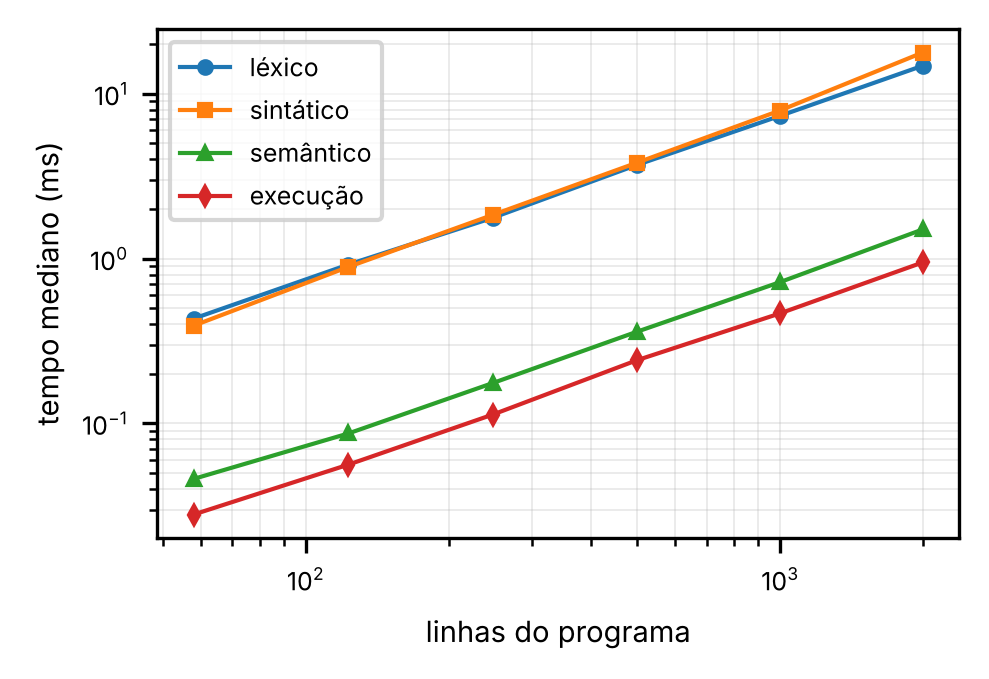
\includegraphics[width=0.95\columnwidth]{fig/fig_bench.png}
\caption{Tempo por fase em função do tamanho do programa (escala log-log).}
\label{fig:bench}
\end{figure}

\subsection{FinFlow em Comparação com Planilha e GPL}

A Tabela~\ref{tab:comp} compara qualitativamente as três abordagens para o mesmo problema (juros sobre um saldo). A comparação é argumentativa, não empírica: não houve estudo com usuários.

\begin{table}[!htbp]
\caption{Comparação Qualitativa}
\label{tab:comp}
\centering
\footnotesize
\begin{tabular}{@{}p{0.27\columnwidth}p{0.20\columnwidth}p{0.18\columnwidth}p{0.18\columnwidth}@{}}
\toprule
\textbf{Critério} & \textbf{Planilha} & \textbf{Python} & \textbf{FinFlow} \\
\midrule
Versionável/testável & difícil & sim & sim \\
Erro \texttt{moeda}+\texttt{\%} & não detecta & não detecta & rejeita \\
Sintaxe do domínio & não & não & sim \\
Exige programar & não & sim & pouco \\
Generalidade & média & alta & baixa \\
\bottomrule
\end{tabular}
\end{table}

\subsection{Decisões de Projeto e Alternativas Descartadas}

A Tabela~\ref{tab:decisoes} reúne as principais decisões, a alternativa considerada e o motivo da escolha, com a seção em que cada uma é discutida. O fio condutor é privilegiar a simplicidade e a detecção precoce de erros em detrimento da generalidade, coerente com uma DSL de escopo restrito.

\begin{table}[!htbp]
\caption{Decisões de Projeto}
\label{tab:decisoes}
\centering
\footnotesize
\setlength{\tabcolsep}{3pt}\begin{tabular}{@{}p{0.27\columnwidth}p{0.26\columnwidth}p{0.36\columnwidth}@{}}
\toprule
\textbf{Escolha} & \textbf{Descartada} & \textbf{Motivo} \\
\midrule
DSL externa & DSL interna em Python & verificar tipos antes da execução (\ref{sec:fund}) \\
Precedência declarada & gramática em níveis (termo/fator) & gramática compacta; risco medido (\ref{sec:precexp}) \\
Reservadas por dicionário & uma regex por palavra & evita competição com \texttt{ID} (\ref{sec:lexico}) \\
Interpretador de AST & geração de código & simplicidade; programas curtos (\ref{sec:interp}) \\
Chaves obrigatórias & blocos opcionais & elimina \textit{else} pendente (\ref{sec:linguagem}) \\
\texttt{escolha} sem \textit{fall-through} & semântica de C & evita erro comum (\ref{sec:linguagem}) \\
Coerção de inteiros & tipagem estrita & ergonomia sem perda de segurança (\ref{sec:semantica}) \\
\bottomrule
\end{tabular}
\end{table}

Uma decisão que merece nota é a da precedência declarada. A alternativa clássica, estratificar a gramática em níveis (\texttt{expressao}, \texttt{termo}, \texttt{fator}), elimina a ambiguidade na própria gramática e dispensa a tabela de precedência, mas multiplica as produções e os estados. A abordagem adotada é mais compacta e legível, ao custo de depender de uma declaração externa à gramática, e foi exatamente essa dependência que o experimento da Seção~\ref{sec:precexp} mostrou ser frágil: um erro de declaração não gera aviso. Uma consequência prática é que a precedência deve ser coberta por teste automatizado, como foi feito.

\subsection{Limitações e Ameaças à Validade}

\textbf{Limitações da linguagem:} não há funções definidas pelo usuário nem estruturas de dados; \texttt{escolha} não faz \textit{fall-through}; os operadores \texttt{e}, \texttt{ou} e \texttt{nao} estão reservados no lexer, mas ainda sem produção na gramática (o \texttt{yacc} emite aviso de tokens sem uso); um literal com ponto decimal é sempre \texttt{moeda}, de modo que não há como escrever um decimal puro; e a variável de controle do \texttt{para} permanece visível após o laço. \textbf{Limitações de implementação:} valores monetários usam ponto flutuante binário, sujeito a erros de arredondamento --- aplicações reais exigiriam aritmética decimal; não há recuperação de erros sintáticos. \textbf{Ameaças à validade:} os experimentos de precedência e desempenho usam programas sintéticos e uma única máquina; o benchmark mede tempo de parede em Python, sensível à carga do sistema; e a afirmação de acessibilidade a analistas financeiros permanece uma hipótese de projeto, sem avaliação com usuários.

\subsection{Reprodutibilidade}

O projeto é distribuído como pacote Python autônomo, com a organização da Tabela~\ref{tab:estrutura}. A execução requer Python 3.10 ou superior e a biblioteca PLY (versão 3.11 ou superior); os testes requerem \texttt{pytest}. Um programa é executado por \texttt{python main.py exemplos/juros.ff} e a suíte por \texttt{pytest}. As figuras deste artigo (arquitetura, AST, saída de execução, AFD e \textit{benchmark}) são geradas por \textit{scripts} a partir da execução real do compilador, e não desenhadas à mão, de modo que mudanças na implementação podem ser refletidas regenerando-as. A saída de depuração do \texttt{yacc}, usada nos experimentos das Seções~\ref{sec:sintatico} e~\ref{sec:precexp}, é obtida ativando o modo \texttt{debug} do gerador.

\begin{table}[!htbp]
\caption{Estrutura do Projeto}
\label{tab:estrutura}
\centering
\footnotesize
\begin{tabular}{@{}p{0.46\columnwidth}p{0.46\columnwidth}@{}}
\toprule
\textbf{Arquivo} & \textbf{Responsabilidade} \\
\midrule
\texttt{finflow/lexer.py} & tokens e erros léxicos \\
\texttt{finflow/parser.py} & gramática, precedência, AST \\
\texttt{finflow/semantica.py} & símbolos e tipos \\
\texttt{finflow/interpretador.py} & execução da AST \\
\texttt{main.py} & interface de linha de comando \\
\texttt{exemplos/*.ff} & seis programas de exemplo \\
\texttt{testes/test\_finflow.py} & nove testes automatizados \\
\bottomrule
\end{tabular}
\end{table}

\section{Conclusão e Trabalhos Futuros}
\label{sec:conclusao}

Este trabalho apresentou a FinFlow, uma DSL externa com tipos nativos \texttt{moeda} e \texttt{percentual}, e seu compilador completo: AFD para a fase léxica, gramática LALR(1) de 29 produções e 68 estados sem conflitos, análise semântica com regras de tipo e interpretador por percurso da AST. A validação mostrou execução correta dos exemplos, rejeição estática da soma de \texttt{moeda} com \texttt{percentual} e custo aproximadamente linear por fase. A contribuição metodológica mais relevante é o experimento de precedência: sobre a gramática real, a ausência de declaração produz 9 conflitos resolvidos por padrão, e um único nível de precedência elimina todos os conflitos mas gera a árvore errada, o que mostra que a ausência de conflitos não garante a semântica pretendida.

Como trabalhos futuros: (i) integrar a API SGS do Banco Central, desacoplada do compilador, alimentando a tabela de símbolos com Selic e IPCA reais por meio dos pontos de extensão já existentes, e calculando, por exemplo, o rendimento real pela relação de Fisher; (ii) incluir operadores lógicos, funções de usuário e aritmética decimal; (iii) incorporar recuperação de erros sintáticos; e (iv) avaliar a linguagem com usuários do domínio financeiro.

\textbf{Esboço da integração prevista.} Com a camada de dados externos, um programa FinFlow poderia usar variáveis pré-declaradas pelo ambiente (aqui hipotéticas, ainda não implementadas) para calcular o rendimento real de uma aplicação:
\begin{minipage}{\columnwidth}\begin{lstlisting}
moeda aplicado = 10000.00;
moeda final = aplicado + aplicado * selic_ano;
imprimir(final);
\end{lstlisting}\end{minipage}\par\smallskip
em que \texttt{selic\_ano}, do tipo \texttt{percentual}, seria preenchida a partir da série 4390 do SGS (composta no período). A análise semântica trataria a variável como declarada e tipada, preservando todas as verificações já existentes.

\begin{thebibliography}{8}
\bibitem{bcb} BANCO CENTRAL DO BRASIL. \textbf{Taxa de juros - Selic acumulada no mês}: série 4390 do Sistema Gerenciador de Séries Temporais (SGS). Brasília: BCB, 2026. Disponível em: \url{https://dadosabertos.bcb.gov.br/dataset/4390-taxa-de-juros---selic-acumulada-no-mes}. Acesso em: 11 out. 2026.
\bibitem{mernik} MERNIK, M.; HEERING, J.; SLOANE, A. M. When and how to develop domain-specific languages. \textbf{ACM Computing Surveys}, New York, v. 37, n. 4, p. 316--344, 2005.
\bibitem{deursen} VAN DEURSEN, A.; KLINT, P.; VISSER, J. Domain-specific languages: an annotated bibliography. \textbf{ACM SIGPLAN Notices}, New York, v. 35, n. 6, p. 26--36, 2000.
\bibitem{aho} AHO, A. V.; LAM, M. S.; SETHI, R.; ULLMAN, J. D. \textbf{Compiladores}: princípios, técnicas e ferramentas. 2. ed. São Paulo: Pearson Addison-Wesley, 2008.
\bibitem{kosar} KOSAR, T.; BOHRA, S.; MERNIK, M. Domain-specific languages: a systematic mapping study. \textbf{Information and Software Technology}, Amsterdam, v. 71, p. 77--91, 2016. DOI: 10.1016/j.infsof.2015.11.001.
\bibitem{peyton} PEYTON JONES, S.; EBER, J.-M.; SEWARD, J. Composing contracts: an adventure in financial engineering. In: ACM SIGPLAN INTERNATIONAL CONFERENCE ON FUNCTIONAL PROGRAMMING, 5., 2000. \textbf{Proceedings} [...]. New York: ACM, 2000. p. 280--292.
\bibitem{kennedy} KENNEDY, A. Types for Units-of-Measure: Theory and Practice. In: HORVÁTH, Z.; PLASMEIJER, R.; ZSÓK, V. (ed.). \textbf{Central European Functional Programming School}: third summer school, CEFP 2009. Berlin: Springer, 2010. p. 268--305. (Lecture Notes in Computer Science, v. 6299).
\bibitem{ply} BEAZLEY, D. \textbf{PLY (Python Lex-Yacc)}. Versão 3.11. [S. l.]: Dabeaz LLC, 2018. Disponível em: \url{https://www.dabeaz.com/ply/}. Acesso em: 11 out. 2026.
\end{thebibliography}

\end{document}
